\documentclass[sigconf]{acmart}
\usepackage{pgfplots}
\usepackage{hyperref}
\pgfplotsset{compat=1.18}
\usepackage{tcolorbox}
\tcbuselibrary{listingsutf8}

\begin{document}

\title{A Comparison of Sinew to Modern Semi-Structured Data Management Systems}

\author{Marie Mellor}
\affiliation{%
  \institution{Rochester Institute of Technology}
  \streetaddress{1 Lomb Memorial Drive}
  \city{Rochester}
  \state{New York}
  \country{USA}}
\email{mhm3244@rit.edu}

\author{Danny Gardner}
\affiliation{%
  \institution{Rochester Institute of Technology}
  \streetaddress{1 Lomb Memorial Drive}
  \city{Rochester}
  \state{New York}
  \country{USA}}
\email{drg5567@rit.edu}

\author{Clinten Hopkins}
\affiliation{%
  \institution{Rochester Institute of Technology}
  \streetaddress{1 Lomb Memorial Drive}
  \city{Rochester}
  \state{New York}
  \country{USA}}
\email{cmh3586@rit.edu}

\acmConference[CSCI-725]{Adv DB: NoSQL/NewSQL}{Fall, 2024}{Rochester, NY}

\begin{CCSXML}
<ccs2012>
   <concept>
       <concept_id>10002951.10002952.10003190.10003192</concept_id>
       <concept_desc>Information systems~Database query processing</concept_desc>
       <concept_significance>500</concept_significance>
       </concept>
 </ccs2012>
\end{CCSXML}

\ccsdesc[500]{Information systems~Database query processing}

\begin{abstract}
    Over the last 10 years, the popularity and use of semi-structured databases has exploded. With this, we take a look back at a promising, at the time, solution to the problem of storing semi-structured data that offered PostgreSQL querying, Sinew. Sinew offered a way to be able to store semi-structured data in PostgreSQL using a custom column materializer and "column reservoir" to be able to store both dense and sparse columns in efficient ways. Since then, offerings from MongoDB and PostgreSQL themselves (through PostgreSQL's \texttt{jsonb} column type) have had continuous development, offering a more competitive solution to these problems. At the time, Sinew outperformed every offering that the authors compared to, so we decided to re-evaluate the system to see if it still holds up today. Overall, the system seems to perform fairly competitively, though has many implementation issues and could benefit from a re-implementation in modern PostgreSQL. 
\end{abstract}

\keywords{Sinew; SQL; Relational Database Management System (RDBMS); NoSQL; JSON; MongoDB; Semi-structured data; Column materialization; Query performance benchmarking; NoSQLBench benchmark suite; Document-oriented database}

\maketitle

\section{Literature Report}
   % Kind of like the related works section of a paper
   We focused on the comparisons between Sinew and the modern database services MongoDB, and PostgreSQL JSON. Our goal in doing this is to see how Sinew compares to modern database systems in aspects such as batch loading, querying, updating and overall performance and scalability. This section will cover the primary works used in our evaluation.

   \subsection{Sinew}

   The main objective of Sinew \cite{Tahara_Diamond_Abadi_2014} is to enable developers to be able to represent data using self-describing formatting while still utilizing SQL and other traditional database systems. It was built to be a middle layer between multi-structured data and a relational database management structure (RDBMS). Sinew acts as an efficient tool able to convert semi-structured data into something stored and maintained in an RDBMS.

   The Sinew system architecture consists of two layers, the use layer and the storage layer. The storage layer allows Sinew to manage and query multi-structured data efficiently. Sinew's schema supports universal relations in which one document corresponds to one row. For every key, value pair from a document, the value will logically get stored in the row and column which corresponds to the document and key. A hybrid approach was used for mapping logical to physical schema to maintain performance benefits, space efficiency and single column serialization. The approach consisted of a combination of "all-physical-column" approach and "all-virtual-column" approach. Using this new hybrid approach, columns for some of the attributes get created while the rest are stored in a special serialized column called the column reservoir. This enables Sinew to maintain the benefits of using physical columns where they're needed while still keeping less frequently accessed keys stored virtually.

   Sinew documents the attribute names, types and storage methods to maintain a correct mapping between logical and physical and make system optimizations possible in a catalog. This catalog keeps track of which keys have been observed, the key type information which has been derived from the data, the number of occurrences of each key, if a column is virtual or physical and a 'dirty' flag. The catalog is split into two parts so Sinew can easily identify logical schema and physical schema.

   A schema analyzer is also used to allow Sinew to adapt to evolving data models and query patterns. This schema analyzer evaluates the current storage schema in order to determine a distribution of physical and virtual columns. This was done to minimize the overall cost of materialization while still maximizing increasing performance rates.

   A column materializer was used to maintain dynamic physical schema by moving data between the column reservoir and physical columns. This materializer was created with the intent of it being a background process that would run only when there are resources available for it within the system. This is where the "dirty column" as previously mentioned comes into play. A dirty column is where some values for a key might exist in the reservoir while others exist in a corresponding physical column. These dirty columns make sure that dirty bits in a catalog are set for that specific column.

   Within the use layer, data is loaded in two steps: serialization and insertion. During the serialization step, the loader first parses each document, making sure that its syntax is valid. After the validation, the document is serialized into the proper format. During the serialization step, the loader also aggregates information about the keys within the dataset such as presence, type and sparsity. This information is then added to the catalog. During the insertion step, all the serialized data is placed into the column reservoir and the dirty flag is set to true in the respective columns. The column data is then moved to physical columns once the dirty bit is picked up which creates the newly loaded data. This was put in place so the system components would remain modular.

   Due to the nature of the hybrid storage, queries must match the physical schema; this is where a query rewriter comes into play. Here, queries are converted into an abstract syntax tree so that they can be validated and later sent to the storage layer to be executed. If any of the column references cannot be validated, the physical column is rewritten.


   \subsection{MongoDB}
   The architecture of MongoDB consists of many features that enable a strong and flexible database. MongoDB is a non-relational document oriented database management system that utilizes a document structure to store its data \cite{Geeks4geeksMongo}. Similar to RDBMS tables, MongoDB uses collections to hold data within the database, the collections are able to store documents which have different fields. Collections in MongoDB are what stores the data whereas documents represent a specific record within a collection. Unlike SQL databases like MySQL, a document with a field that might not exist in the database does not cause any errors \cite{Mongo-Medium}.
  
   As of 2014, MongoDB's default storage engine became WildTiger \cite{Mongo-Medium}. WildTiger enabled two concurrent writes to update different documents in the same collection without the need for serialization. This feature that was not possible with the original release of MongoDB. The Binary-JSON (BSON) objects in WildTiger are compressed and stored in a hidden index where BSON pairs stores any recordIDs. This increases the performance greatly by reducing the number of I/O transactions.


   The process by which MongoDB scales its data is necessary in order to meet any growing demands of an application or database. MongoDB supports two types of scaling: horizontal and vertical \cite{Mongo-scalability}. Horizontal scaling, or scaling down, is done by distributing the data across multiple nodes where each node is responsible for storing portions of the data. This is achieved by sharding, a mechanism that involves partitioning a database into smaller parts called 'shards'. These shards are hosted on a separate server forming what is known as a shard cluster. Vertical scaling, or scaling up, is the act of increasing the capacity of a single server by adding CPU, RAM, or other storage resources. In terms of MongoDB, this would mean upgrading the hardware to something more powerful. This may prove to be effective overall but has its own limitations.
  

   \subsection{PostgreSQL JSON}
    PostgreSQL architecture \cite{PostgresMedium} is a combination of shared memory, background processes, and data files. The shared memory contains a shared buffer, and a WAL buffer. The shared buffer is responsible for minimizing disk input/output so long as it is able to minimize contention when accessed by multiple users. The shared buffer needs to be large enough so that it may be accessed quickly. The shared buffer should keep any frequently used blocks as long as possible. The WAL buffer is used to store changes in the database temporarily in a WAL file. The four main process types that Postgres hosts are: Postmaster, background, backend, and client. The Postmaster process creates the backend processes for the client connections and is the overall parent process for the rest of the processes. The background processes all serve different functions and play a major role in database management. The backend process executes queries before returning the results to the user. This task is reliant on local memory.

    In terms of scalability, Postgres scaling\cite{Postgres-scalable} requires the understanding and proper implementation of PostgreSQL horizontal scaling as well as vertical scaling. PostgreSQL is kept accessible by high availability (HA) regardless of hardware failures or software crashes. This type of HA implementation requires replication, failover, load balancing and continuous monitoring.


\section{Completed Work}
% TODO: What is the plan for this section, I assume just convert it into a "Completed Work" of some kind?
    \subsection{Sinew Implementation}
    The main task of this project was ensuring that the Sinew code was able to still load and run in the modern day. In the original paper's implementation of Sinew they used Postgres as the underlying database \cite{Tahara_Diamond_Abadi_2014}. For this project, we aimed at simply getting the system to run with the version it was created with (9.3.0). The Sinew repository included multiple bash and make files that perform the initial setup, install the database, and perform some basic tests.

    The biggest challenge with implementing Sinew was the lack of documentation in the repository. The initial README file provided no information on how to configure, initialize, or run the system. This left us with a daunting task of having to parse through each file in the repository to understand its function and how it impacted the overall system. In addition to no overarching documentation, the plentiful bash files in the repository were similarly left undocumented, which forced us to analyze each file to understand each one's intended purpose and the order in which to execute them. As we analyzed the original source code we attempted to remedy this situation, creating our own documentation for the repository which will allow future users to reproduce our implementation easily.

    We updated the initialization and startup files so that the project can be run on a WSL Ubuntu Linux instance. After the changes to these files the necessary software was able to be installed on the instance and build a test database hosted on postgres. Diving into the Sinew code, there seemed to be many missing files in the repository that were necessary in order to implement the system, including configuration files and the original data directories. The document parser, schema analyzer, and the coulumn upgrader were developed as custom Postgres extensions, which required a global configuration file that was missing. Thankfully, the original developers created options in their makefiles to utilize PGXS, the Postgres extension makefile format, which is a built-in feature since version 8.0. This framework provided many basic makefile configurations that were feasbile to run on this project. After editing the installation bash file to utilize PGXS, the custom extensions were able to be installed. In addition to the installation script, we made slight modifications to the premade run script that allowed the postgres server to function, allowing Sinew to run.

    As for the Sinew source code, limited modifications were needed to ensure the system ran as intended. These extension files were developed in C to implement the necessary functions that Sinew needed. Upon the inital tests, the repository was having segmentation faults due to a buffer overflow occuring during the document serialization. A minor fix was implemented to correct this error and allowed for documents to be properly serialized and loaded into the database. While the main memory issue was resolved to allow Sinew to function properly, further analysis showed many other memory leaks and issues within the repository. These errors did not compromise the system completely, but as shown later in the results it prevented Sinew from operating as fully as it once had. It was not determined whether these issues had been there from the start or were the result of outdated C code.

    To load data into the Sinew database, there was a bash script that extracted the data files and exectued stored SQL queries that invoked the serialization function. This would store all loaded data as serialized documents in the column reservoir. This script was modified to locate the directory where our new dataset was stored and perform the SQL load queries. These loading queries also needed slight modifications in order to locate our new data. After these changes were made the system was able to effectively load the database.

    Similarly to the benchmark loading functions, the system test files were outdated and needed to be updated in order to effectively test the benchmark queries. The bash script was updated in order to execute the given query files and store their runtime in an output directory. Additionally, we added the ability to load and clear the database from this query to simplify the testing process. This testing script also performed the upgrades that created physical columns from the reservoir that allowed for the SQL functions to be exected on the table. This upgrade function was in the form of SQL queries that utilized user-defined functions provided by the original developers. This file was modified to use the correct data table that the queries were executed on. Finally, the query SQL scripts required some syntax updates to streamline the testing process. After these modifications, Sinew was able to perform the necessary tasks needed for this project.

    \subsection{MongoDB Benchmark}
    In the original paper the authors compared the implementation of Sinew against MongoDB and Postgres JSON. During this phase, we also started configuring the MongoDB benchmark system. We will expand on that below. During these experiments the database systems were evaluated on their performance of varying queries from the NoBench NoSQL benchmark suite \cite{NoSQLBench}. Testing on Mongo was pretty straightforward in terms of implementation. \cite{NoSQLBench} has pre-written queries for Mongo version 2.0.0, but as the program has evolved, some of those queries were out-of-date. The most obvious being Queries 10 and 11; for those queries, we had to re-implement the queries with Mongo's \texttt{aggregate} framework, released in Mongo 2.2, with support for \texttt{\$lookup} operations added in Mongo 6.0  \cite{Done2023}.

    \subsection{PostgreSQL JSON Benchmark}
    As mentioned in the original paper, PostgreSQL 9.3 was one of the systems that Sinew was compared to in terms of performance. Through storing the data in \texttt{jsonb}, we were able to load all 16 million rows to the database and recreate the queries of the original paper with little to no issue. However, many advancements have been made in the last ten years since the paper was written. For our experiments, we recreated the queries from the paper using a much more modern version of the database, PostgreSQL 14.4. A significant difference between 9.3 and 14.4 is that \texttt{jsonb} was not supported at the time of the original paper~\cite{PostgtesVersions}. This proves to be a significant detail since we stored our data in \texttt{jsonb} format within the database. 

    Due to \texttt{jsonb} not being available at the time the paper was originally published, this also meant that \texttt{jsonb}-modifying operators and functions had also not been available. Without these advancements, we would not have had access to the operators and functions that enable queries to delete, modify, and insert into \texttt{jsonb} values. It is apparent that PostgreSQL 14.4 also has many improvements regarding performance that were not available at the time of the initial paper such as has aggregation being able to use disk as well as parallel merge joins and queries. 

    \subsection{NoSQLBench}
    In the original paper the authors used the NoBench NoSQL benchmark suite to run their analysis. As this is a closed-source tool, we did not have access to it for our analysis. In lieu of that, we chose to use an existing, open-source, tool that has a similar feature set and worked well for our use case; this tool was NoSQLBench \cite{NoSQLBench}. 
    
    This tool was built for NoSQL databases like MongoDB, Neo4J, Pulsar, etc. \footnote{\url{https://github.com/nosqlbench/nosqlbench/tree/main/nb-adapters}}, but did not have any support for PostgreSQL JSON or Sinew. This meant we could not use this tool for our entire testing suite. Our solution was to generate all of the required data (per the NoSQL Benchmark's specifications \cite{Chasseur_Li_Patel_2013}) and then manually run the queries on the environments ourselves. Sinew already had this feature built into the repo \footnote{\url{https://github.com/danieltahara/sinew/tree/master/benchmark/system/document}}, so we were able to easily run that (once our refactoring was done). MongoDB was easy enough to implement as we just set up a JavaScript file with all of our queries and used JavaScript's timers to track the time. PostgreSQL was also relatively simple as we were able to open a connection with a Python script and run the queries directly. 

\section{Experiments}

Our experiments try to mimic the experiments done in \cite{Tahara_Diamond_Abadi_2014} by replicating the queries created in \cite{Chasseur_Li_Patel_2013}. We ran all of our testing on isolated Ubuntu 24.04.1 instances. The system had a 3.60 GHz, 6-Core, AMD Ryzen 5 3600 processor with 16 GB of memory and 2 TB of NVMe solid-state storage. We executed each of the 11 queries (excluding the update task defined in \cite{Tahara_Diamond_Abadi_2014}), at least 4 times and took the average of the results. 

\subsection{Load Times}

\begin{figure}[!t]
\centering
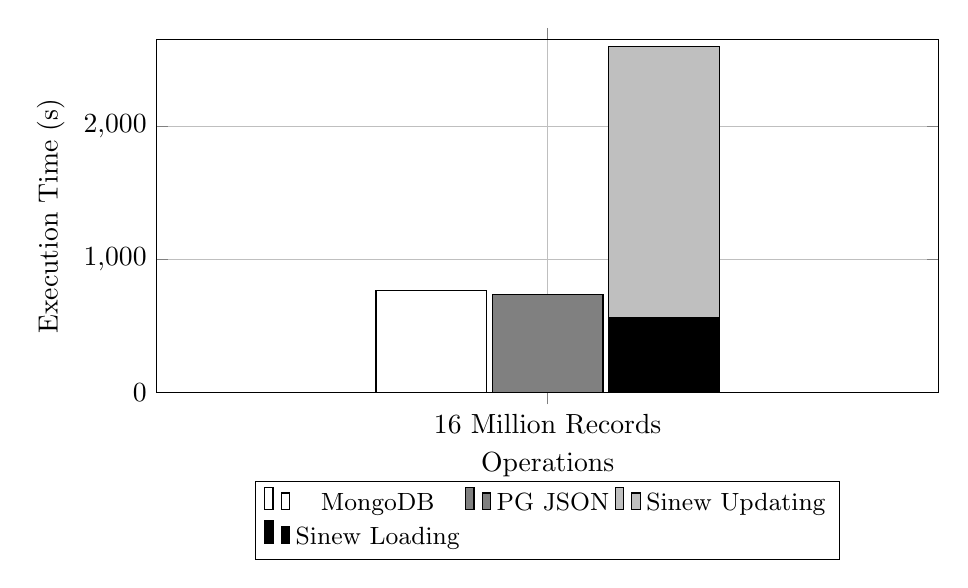
\begin{tikzpicture}
\begin{axis}[
    ybar, % Regular bar chart
    symbolic x coords={16 Million Records},
    xtick=data,
    xlabel={Operations},
    ylabel={Execution Time (s)},
    ymin=0,
    ymax=2650,
    legend style={at={(0.5,-0.25)}, anchor=north, legend columns=3, font=\small},
    bar width=40pt,
    width=0.95\columnwidth,
    height=0.5\columnwidth,
    grid=major,
    enlarge x limits=0.4, % Adds space between grouped bars
]

% MongoDB Bar
\addplot[fill=white, bar shift=-42pt] coordinates {(16 Million Records, 763.76)};
\addlegendentry{MongoDB}

% PG JSON Base
\addplot[fill=gray, bar shift=+0pt] coordinates {(16 Million Records, 734.35)};
\addlegendentry{PG JSON}

% PG JSON Base
\addplot[fill=lightgray, bar shift=+42pt] coordinates {(16 Million Records, 2598.029413)};
\addlegendentry{Sinew Updating}

% PG JSON Additional (stacked on top of the gray bar)
\addplot[fill=black, bar shift=+42pt] coordinates {(16 Million Records, 565.169413)};
\addlegendentry{Sinew Loading}

\end{axis}
\end{tikzpicture}
\caption{Load Time}
\label{fig:load_time}
\Description[A chart showing the load times of each system.]{This chart shows the total time it took to load the data into each system. For MongoDB, this was about 760 seconds; for PG JSON, this was about 730 seconds; for Sinew, there was an initial load time of about 560 seconds, but then an additional "update" time of about 2,530 seconds, during which the data was converted into a usable format.}
\end{figure}

The initial paper evaluated the load time and data sizes of all of the evaluated systems; our evaluation only looked at the total load time. When comparing our results to \cite{Tahara_Diamond_Abadi_2014}, we noticed an interesting discrepancy in the Sinew load time. Sinew, seemed to perform as well as MongoDB in its initial loading, while only being twice as slow as PG JSON. When we ran our evaluation, we got similar load times for Sinew, actually beating the PG JSON load times, but we noticed there was a secondary operation that took place before the data was actually queryable. This "update" step pushed the total time to over three times longer than both the MongoDB and PG JSON loading. While this is not technically the "loading" of the data, and in theory, this updating could happen in the background while Sinew is running (as described in section 5 of \cite{Tahara_Diamond_Abadi_2014}), in the current implementation of Sinew, this is not possible, so the update step is required for any querying to take place. These are noted as separate operations in \autoref{fig:load_time}, but we wanted to mention it as it impacts the results of this section greatly.

\subsection{Projections}

\begin{figure}[!t]
\centering
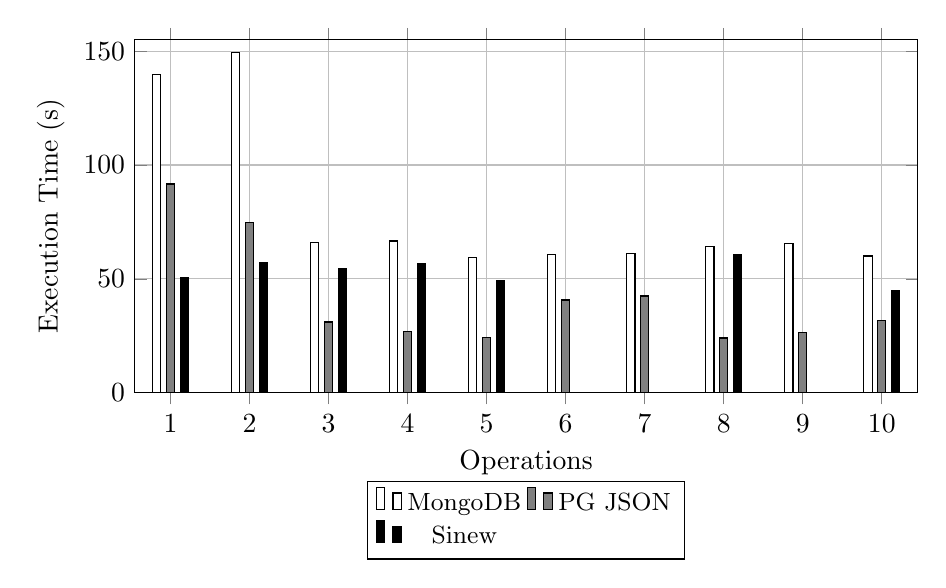
\begin{tikzpicture}
\begin{axis}[
    ybar,
    symbolic x coords={1, 2, 3, 4, 5, 6, 7, 8, 9, 10},
    xtick=data,
    xlabel={Operations},
    ylabel={Execution Time (s)},
    ymin=0,
    ymax=155,
    legend style={at={(0.5,-0.25)}, anchor=north, legend columns=2, font=\small},
    bar width=3pt,
    width=0.95\columnwidth,
    height=0.5\columnwidth,
    grid=major,
    enlarge x limits=0.05,
]

% Data for MongoDB
\addplot[fill=white] coordinates {(1, 139.8) (2, 149.4) (3, 66.0) (4, 66.6) (5, 59.4) (6, 60.6) (7, 61.2) (8, 64.2) (9, 65.4) (10, 60)};
\addlegendentry{MongoDB}

% Data for PG JSON
\addplot[fill=gray] coordinates {(1, 91.62) (2, 74.64) (3, 31.02) (4, 26.82) (5, 24.12) (6, 40.68) (7, 42.42) (8, 24.0) (9, 26.34) (10, 31.56)};
\addlegendentry{PG JSON}

% Data for Sinew
\addplot[fill=black] coordinates {(1, 50.52) (2, 56.94) (3, 54.6) (4, 56.58) (5, 49.14) (8, 60.84) (10, 44.94)};
\addlegendentry{Sinew}

\end{axis}
\end{tikzpicture}
\caption{NoSQLBench Query Performance (Q1-Q10)}
\label{fig:queries_1_10}
\Description[A chart showing the total execution times of queries 1 through 10.]{This chart shows the total execution times of queries 1 through 10. For MongoDB, the queries took: 139.8 seconds, 149.4 seconds, 66.0 seconds, 66.6 seconds, 59.4 seconds, 60.6 seconds, 61.2 seconds, 64.2 seconds, 65.4 seconds, and 60 seconds. For PG JSON, the queries took: 91.62 seconds, 74.64 seconds, 31.02 seconds, 26.82 seconds, 24.12 seconds, 40.68 seconds, 42.42 seconds, 24.0 seconds, 26.34 seconds, and 31.56 seconds. For Sinew, some queries could not execute due to memory issues. Due to this, queries 1 through 5, query 8, and query 10 took, respectively: 50.52 seconds, 56.94 seconds, 54.6 seconds, 56.58 seconds, 49.14 seconds, 60.84 seconds, 44.94 seconds.}
\end{figure}

Queries 1 through 4 are simple data projections of top-level, nested, and sparse keys. \autoref{fig:queries_1_10} shows that overall MongoDB did perform the slowest on the data provided. For queries 1 and 2, Sinew performed almost one-third of the time, compared to MongoDB. PostgreSQL followed closely behind Sinew, with its performance increasing for Query 2 (the nested key lookup).

Regarding the sparse queries, Sinew lost its top spot and PostgreSQL took the lead in terms of execution time. PostgreSQL performed in about half the time Sinew and MongoDB took to complete the query, and was the only system to see an improvement when running Query 4 (a sparse key with double the cardinality of Query 3). Below we can see the difference in implementation for each of those queries:

\noindent
MongoDB:
\begin{tcolorbox}[colback=gray!10, colframe=gray!50, sharp corners, boxrule=0.1mm]
\begin{verbatim} 
db["main"].find({
  "$or":[ 
    { "sparse_XX0" : {"$exists" : True} },
    { "sparse_YY0" : {"$exists" : True} } 
  ] 
}, ["sparse_XX0", "sparse_YY0"])
\end{verbatim}
\end{tcolorbox}

\noindent
PostgreSQL JSON:
\begin{tcolorbox}[colback=gray!10, colframe=gray!50, sharp corners, boxrule=0.1mm]
\begin{verbatim} 
SELECT 
    data ->> 'sparse_XX0' AS sparse_1,
    data ->> 'sparse_YY0' AS sparse_2
FROM main
WHERE data ? 'sparse_XX0' OR data ? 'sparse_YY0';
\end{verbatim}
\end{tcolorbox}

\noindent
Sinew:
\begin{tcolorbox}[colback=gray!10, colframe=gray!50, sharp corners, boxrule=0.1mm]
\begin{verbatim} 
SELECT 
    document_get_text(data, 'sparse_XX0'),
    document_get_text(data, 'sparse_YY0') 
FROM main;
\end{verbatim}
\end{tcolorbox}

\subsection{Selections}

Queries 5 through 9 were evaluations on both "rifle-shot" selection (Query 5) and range selection. PostgreSQL maintained its leadership in query 5, finding the matching record in under half the time of the other systems. 

Queries 6, through 9 were disappointing when it came to evaluating the Sinew. After spending weeks to get the Sinew implementation\footnote{\url{https://github.com/danieltahara/sinew}} running, we ran into memory issues that caused queries 6, 7, and 9 to fail every time. The output seemed to be complaining about missing "chunks" but due to the old version of PostgreSQL, we were struggling to find a usable solution to this issue. We eventually decided that these queries were just unexecutable without further development. Of the results we were able to produce, PostgreSQL was again outperforming MongoDB for every query and the gap between Sinew and MongoDB was closing, with the total time being within half a second.

\subsection{Joins and Aggregations}

\begin{figure}[!t]
\centering
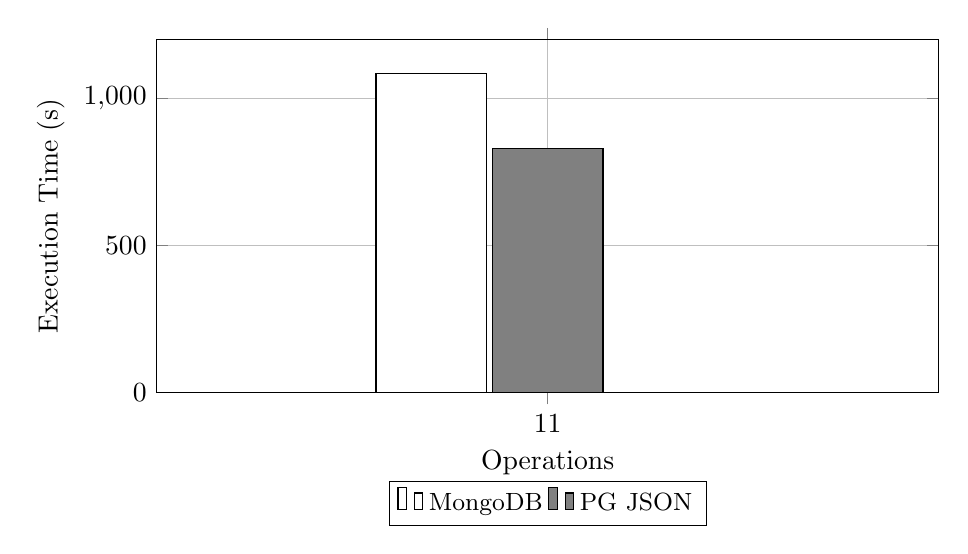
\begin{tikzpicture}
\begin{axis}[
    ybar,
    symbolic x coords={11},
    xtick=data,
    xlabel={Operations},
    ylabel={Execution Time (s)},
    ymin=0,
    ymax=1200,
    legend style={at={(0.5,-0.25)}, anchor=north, legend columns=2, font=\small},
    bar width=40pt,
    width=0.95\columnwidth,
    height=0.5\columnwidth,
    grid=major,
    enlarge x limits=0.05,
]

% Data for MongoDB
\addplot[fill=white, bar shift=-42pt] coordinates {(11, 1084.8)};
\addlegendentry{MongoDB}

% Data for PG JSON
\addplot[fill=gray, bar shift=+0pt] coordinates {(11, 829.8)};
\addlegendentry{PG JSON}

\end{axis}
\end{tikzpicture}
\caption{NoSQLBench Query Performance (Q11)}
\label{fig:query_11}
\Description[A chart showing the total execution times of query 11.]{This chart shows the total execution times of query 11. For MongoDB, this was about 1,080 seconds; for PG JSON, this was about 830 seconds; for Sinew, the program could no longer run the query as it was hitting memory errors on our system. We assume this is probably due to the version of PostgreSQL no longer being supported, but further investigation may find different results.}
\end{figure}

Queries 10 and 11 test the performance of \texttt{GROUP BY} and \texttt{JOIN} operations in the PostgreSQL and Sinew implementations and the \texttt{\$group} and \texttt{\$lookup} operations in MongoDB. \autoref{fig:queries_1_10} shows the performance of Query 10 between all three systems. MongoDB was the slowest, even though Query 10 was the fastest query MongoDB was able to perform (with an average time of exactly one minute). Sinew was about 15 seconds faster than MongoDB and PostgreSQL was the fastest with under 30 seconds. The \texttt{jsonb} column type seems to have very high performance, even without indexing enabled.

Query 11's results are shown in \autoref{fig:query_11}. The results here were a bit disappointing. Sinew was again struck by the memory issues described in section 3.3. The system was unable to produce any results over any of our executions for this query and would always complain of "missing chunks." Of the results we were able to produce, PostgreSQL outperformed the MongoDB implementation by a little over 15\%. 

Though it did not complete, we wanted to show the implementation differences for these queries to highlight Sinew's simple syntax.

\noindent
MongoDB:
\begin{tcolorbox}[colback=gray!10, colframe=gray!50, sharp corners, boxrule=0.1mm]
\begin{verbatim} 
db["main"].aggregate([
  {
    $match: {
      num: { $gte: XXXXX, $lte: YYYYY }
    }
  },
  {
    $lookup: {
      from: "main",
      localField: "nested_obj.str",
      foreignField: "str1",
      as: "matchedDocs"
    }
  }
]);
\end{verbatim}
\end{tcolorbox}

\noindent
PostgreSQL JSON:
\begin{tcolorbox}[colback=gray!10, colframe=gray!50, sharp corners, boxrule=0.1mm]
\begin{verbatim} 
SELECT 
    c.data ->> 'nested_obj' ->> 'str',
    jd.data ->> 'str1' AS str1
FROM main jd
LEFT JOIN main od
    ON jd.data -> 'nested_obj' ->> 'str' 
        = od.data ->> 'str1'
WHERE (jd.data ->> 'num')::int >= XXXXX
AND (jd.data ->> 'num')::int <= YYYYY;
\end{verbatim}
\end{tcolorbox}

\noindent
Sinew:
\begin{tcolorbox}[colback=gray!10, colframe=gray!50, sharp corners, boxrule=0.1mm]
\begin{verbatim} 
SELECT *
FROM main t1 INNER JOIN main t2
    ON (document_get_text(t1.nested_obj, 'str') 
        = t2.str1)
WHERE left.num BETWEEN XXXXX AND YYYYY;  
\end{verbatim}
\end{tcolorbox}

\section{Conclusion}
Even 10 years since its development, Sinew still shows competitiveness handling semi-structured data with modern database systems. While it does not beat its competitors as strongly as before, it was able to keep up with these systems that have gone through major overhauls in the last few years. Sinew remains a novel method to perform relational transactions on document-based data. Its implemntation could definitely be improved upon, as in our investigation we had to fix glaring errors and were unable to completely remedy some. For Sinew to be as effective today as it was at its creation, it would need a major overhaul in its source and testing code. This would be an unreasonable task if the goal were to use this in production, as many other effective database systems are avaialable today. For future research work it would be a fascinating project to update this code to modern Postgres and C implementations. When utilizing the full capabilities of these systems today, Sinew could very well see its performance surpass its competitors once again.

\bibliographystyle{acm}
\bibliography{final_references}

\end{document}